\documentclass[preprint]{aastex}
\usepackage{amsmath, amsfonts, amssymb}
\usepackage{fullpage}

\begin{document}
\title{Characterizing Beam Size and Squint at the ATA}
\author{Keaton J. Burns, Peter Williams, Geoffrey Bower \\ \today}

\begin{abstract}
We present a study of primary beam size and squint in the antennas and
feeds at the Allen Telescope Array (ATA), based on weekly Hex-7
observations from STARTDATE to ENDDATE.  A relational database of beam
parameters was created, which reduces the results of an upgraded and
automated hex analysis pipeline.  A Python visualization tool was
developed to efficiently interface with the squint database and search
for correlations in this large dataset.  We find that...  .
\end{abstract}

\tableofcontents


%%%%%
\section{Introduction}\label{s.intro}
ATA telescope calibrations are accomplished through observing known
radio point sources to determine the system temperature, pointing
centers, and beam shape for each antenna.  One parameter of interest
from these observations is telescope squint, which describes the
offset of the Y polarization pointing center from the X polarization
pointing center, in azimuth and altitude.  Knowledge of each
telescope's squint is useful for assessing the reliability of data
from each polarization based on each telescope's pointing model
(i.e.~for large-squint telescopes, pointing models based on X
polarization pointing centers yield suboptimal Y polarization
data). Studying telescope squint also provides insights into the
strengths and limitations of the offset-Gregorian dish and
log-periodic feed designs used at the ATA, and may be useful for
directing future telescope development.  Our aims in this project
included isolating the cause of the squint to the feed or dish,
studying the effects of feed upgrades on the squint, and assessing the
stability of a telescope's squint with changes in frequency and time.


%%%%%
\section{Data Collection}\label{s.datacollection}

\subsection{Hex7 Observations}\label{ss.observations}
The Hex-7 observing routine consists of a central pointing at a known
radio point source and six pointings in a hexgonal pattern around the
source, and are generally completed once each week.  Flux measurements
are recorded for each antenna and polarization (antpol). Observations
have most often been taken using two correlators at 700 \& 1430, 2009
\& 3140, and 5000 \& 7600 MHz, with the focus set for the higher of
each pair of frequencies, and the hexagonal observations at the
nominal primary beam FWHM for that frequency\footnote{According to
  which precise rule?  Harp 3.5/fghz?}.  Each of these three
observations takes roughly 18 minutes \footnote{cite? hex
  proposals?}. We expect data at 1430 and 3140 MHz to be the most
accurate, since these observations are the most numerous and were in
focus. The radio sources 3c48, 3c138, 3c147, and 3c286 have been used.

\subsection{Data Reduction}\label{ss.reduction}
Part of the Hex-7 data reduction includes fitting a two-dimensional
Gaussian function to the relative gains at each of the seven pointings
for each antpol.  This procedure provides a measurement of the actual
primary beam of the telescope at the observed frequency with respect
to the contemporary pointing model.  The center and width
uncertainties, the reduced Chi-squared value of the fit and the system
equivalent flux density (SEFD) for each antpol were also calculated.

The reduced beam parameters from all Hex-7 runs were added to a
relational database for analysis.  The query script returns any
requested parameters filtered by conditions on any others.  Derived
data such as squint magnitudes and angles, and their respective
uncertainties, are derived during retrieval.

\subsection{Flagging}\label{ss.flagging}
A data-flagging mechanism was implemented to exclude bad data from
future analyses.  To remove bad observations, and particularly poor
reduction fits, observations with frequency normalized squint or width
components in the top percent, or uncertainties in the top two
percent, were removed.  Observations in the top two percent of SEFD,
and top ten percent of the Gaussian fit Chi-squared value were also
flagged.  The Chi-squared cutoff is at a significantly lower
percentile, as it is a direct indicator of the convergence of the
Gaussian fits, and there were a significant number of very high
outliers in this parameter, as shown in Fig.~\ref{fig.dist_sumchisq}.

Nearly all observations at 700 MHz, the lowest observed frequency,
were flagged under these conditions, so the remaining observations
were also excluded.  Additionally, data at 3140 MHz revealed a strong
beam size and shape dependence on the observed source, seemingly
caused by source confusion, prompting us to flag all but the 3c48
observations (see Fig.~\ref{fig.source_confusion}).  After flagging,
1309 observations remained.

\begin{figure}[h!]
\begin{center}
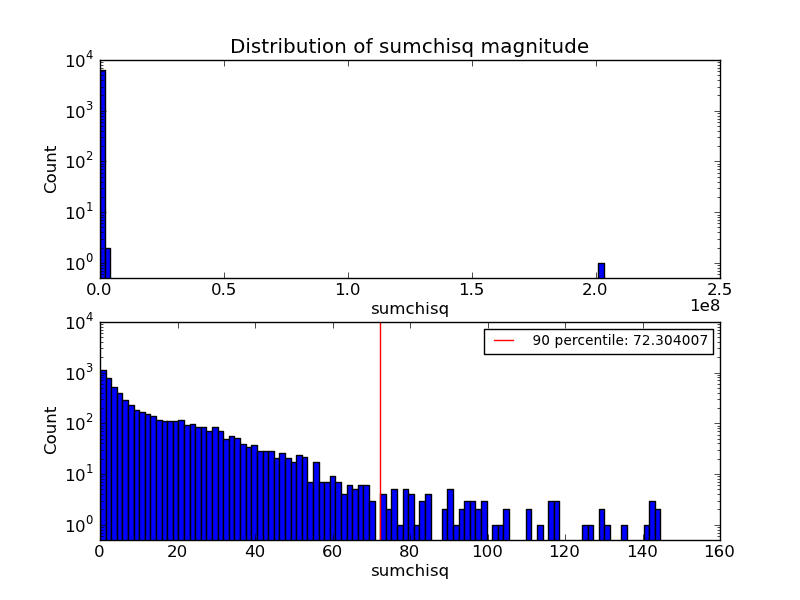
\includegraphics[width=0.7\textwidth]{images/dist_sumchisq.png}
\caption{Top: Distribution of Chi-squared values for 2d Gaussian
  primary beam fits across all Hex-7 observations.  Bottom: Zoom-in at
  flagging cutoff at the 90th percentile. \label{fig.dist_sumchisq}}
\end{center}
\end{figure}

\begin{figure}[h!]
\begin{center}
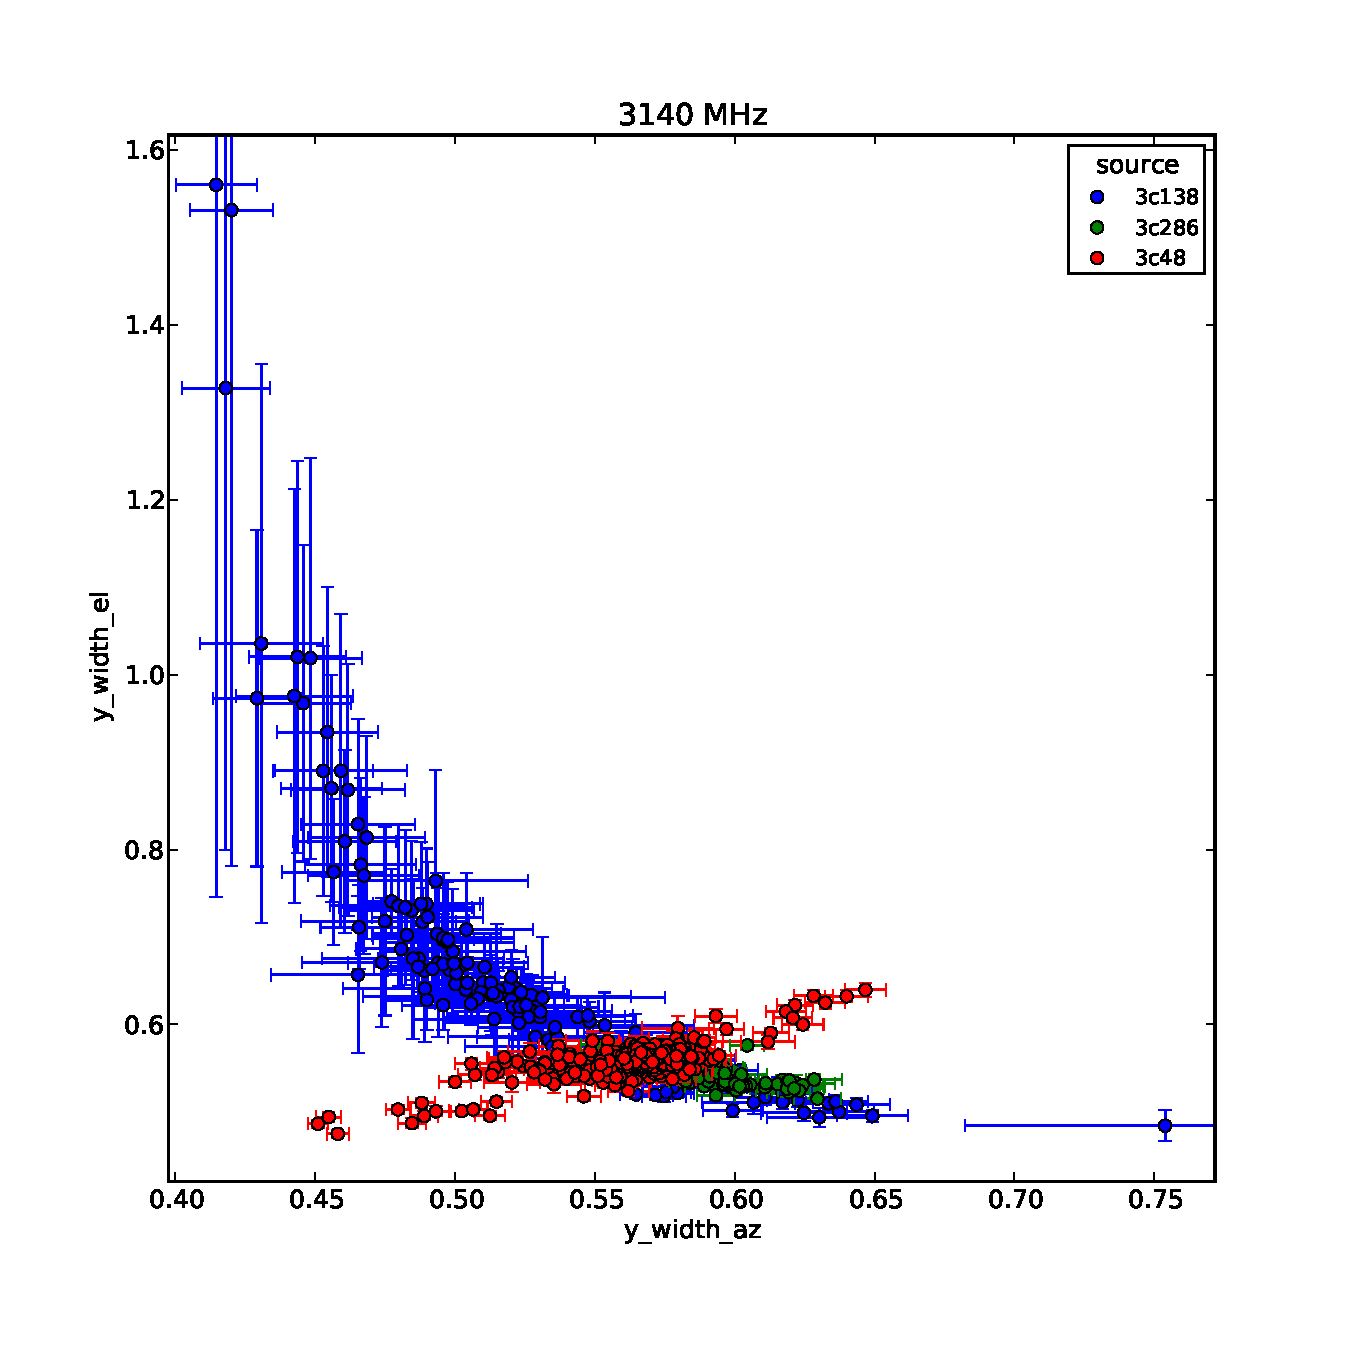
\includegraphics[width=0.8\textwidth]{images/source_confusion.pdf}
\caption{Source confusion in 3140 MHz observations.  Source 3c48 used
  for analysis. \label{fig.source_confusion}}
\end{center}
\end{figure}


%%%%%
\section{Analysis and Results}\label{s.results}

\subsection{Primary Beam Size}\label{ss.beamsize}
Scatterplots depicting the primary beam shape (best-fit 2d Gaussian
elevation width vs azimuthal width) for the X and Y polarizations are
depicting in Figs.~\ref{fig.x_widths} and \ref{fig.y_widths}
respectively, and Table \ref{tab.widths} gives the means and standard
deviations of these values.  We find general agreement with the
approximate results of Harp et al. 2011\cite{Harp2011}, namely $FWHM
\approx 3.5^{\circ} / f_{GHz}$.

\begin{table}[!h]
\begin{center}
\begin{tabular}{|c|c|c|c|} \hline
Polarization & Direction & Mean [$^{\circ} / f_{GHz}$] & St. Dev \\
\hline
\hline
X & El & 3.663 & 0.245\\
\hline
X & Az & 3.443 & 0.216 \\
\hline
Y & El & 3.568 & 0.331 \\
\hline
Y & Az & 3.568 & 0.303\\
\hline
\end{tabular}
\caption{Best-fit primary beam width averages \label{tab.widths}}
\end{center}
\end{table}

\begin{figure}[h!]
\begin{center}
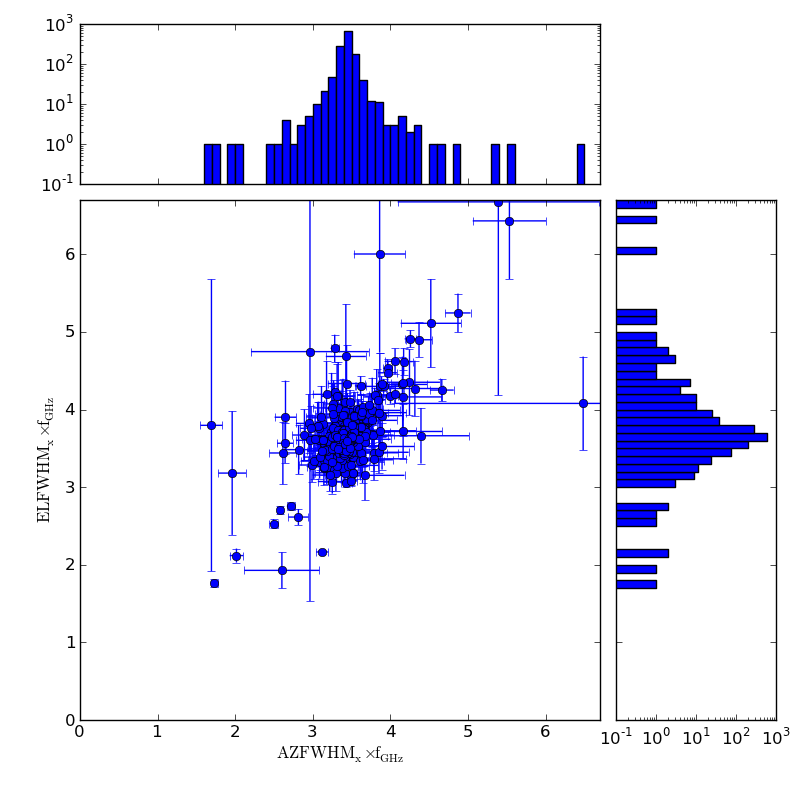
\includegraphics[width=0.8\textwidth]{images/x_widths.png}
\caption{X polarization primary beam widths. \label{fig.x_widths}}
\end{center}
\end{figure}

\begin{figure}[h!]
\begin{center}
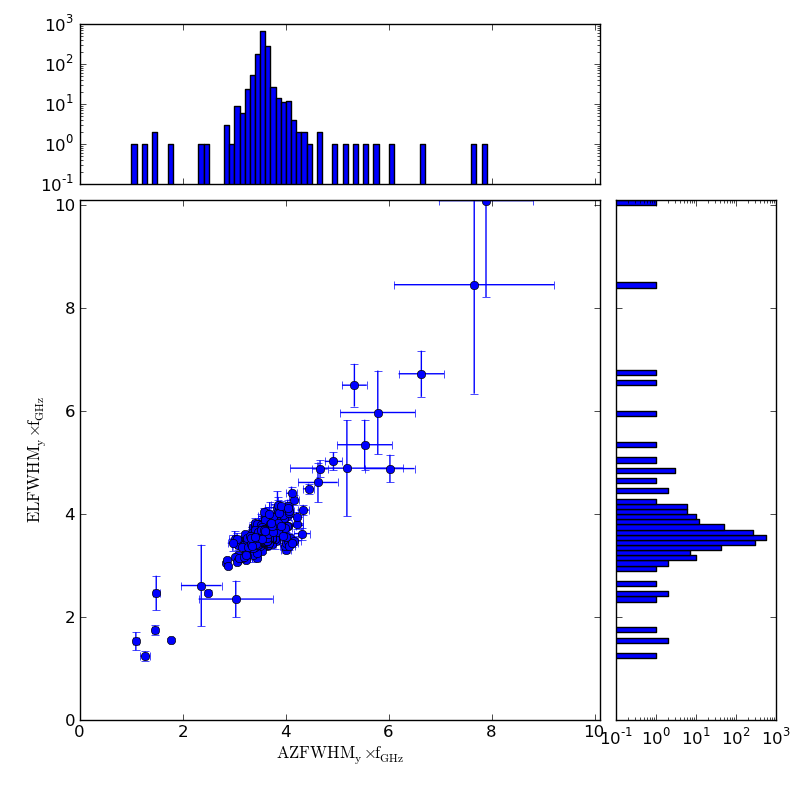
\includegraphics[width=0.8\textwidth]{images/y_widths.png}
\caption{Y polarization primary beam widths. \label{fig.y_widths}}
\end{center}
\end{figure}

\subsection{Squint: Temporal Variation}\label{ss.temporal}

\subsection{Squint: Feed vs. Antenna}\label{ss.antfeed}

\subsection{Squint: Effects of Feed Revisions}\label{ss.revisions}

\subsection{Squint: Frequency Dependence}\label{ss.freq}
To study the effects of frequency on squint, for each antfeed, we
calculated the median squint magnitude, across all observing runs, at
each observing frequency.  We then performed a linear least-squares
fit on the log of the magnitude and the log of the frequency; the
slope of this fit represents the best fitting power-law index $x$,
assuming $|\vec{S}| \propto f^x$.

OR

To study the effects of frequency on squint, for each antfeed, we
performed a linear least-squares fit on the log of squint magnitude
and the log of frequency for each observing run.  The slope of this
fit represents the best fitting power-law index $x$, assuming
$|\vec{S}| \propto f^x$.  We then took the median power-law index
across all observing runs for each antfeed.

The best fitting linear slope was similarly computed for each antfeed
(fitting squint magnitude to frequency, assuming a power-law index of
1).  Histograms of these indices and slopes are displayed in figure
NEEDREF.  The same plots were generated with the data separated by
feed revision.  We notice substantial spread in the power-law indices,
mainly between 0 and -2.  We note that the data for for feed revision
3 show less spread (0 to -1) than the other revisions.

%%%%%
\section{Conclusions}\label{s.conclusions}


%%%%%
\bibliographystyle{plain}
\bibliography{ATA.bib}

\end{document}
